%---------------------------------------------------------------------
\chapter{Experimentation}
%---------------------------------------------------------------------

This chapter reports one controlled A/B experiment. The factor varied is the re-planning loop, which
is the main agentic element of LoomTrace: in variant~A the grader may never send control back to the
planner, and in variant~B, the default configuration, it may do so up to two times. The experiment
answers whether this loop is worth its cost.

\section{Hypothesis}

Allowing the agent to re-plan and retrieve again when the first registry lookup or document search is
inconclusive (variant~B) will increase verdict accuracy compared with a single planning pass
(variant~A), without increasing false \emph{Supported} verdicts, at a latency cost of less than one
second per case.

The hypothesis is falsifiable in three ways: accuracy could fail to rise, the loop could introduce
false \emph{Supported} verdicts by resolving names too permissively, or the extra iteration could cost
more than one second.

\section{Experimental Setup}

\paragraph{Variants.} Variant~A sets the maximum number of planning iterations to one. Variant~B sets it
to three, the value used in all other chapters. In both variants, the first iteration is identical: an
exact registry match and an unfiltered document search. Only variant~B can perform the second
iteration, which resolves aliases and filters the search to the resolved product.

\paragraph{Fixed factors.} The code, the graph, the tools, the reference data, the BM25 parameters,
the grading formula, the guardrail thresholds and the 45-case golden set were identical for both
variants. No language model was used in either variant.

\paragraph{Procedure.} The script \texttt{loomtrace/experiments.py} ran both variants on all 45 cases,
alternating A and B within each of three repetitions, so that any warm-up effect affects both variants.
For each case it recorded the verdict, the number of iterations, the number of tool calls, the number
of node executions and the wall-clock time.

\paragraph{Metrics.} Verdict accuracy, macro-F1, false \emph{Supported} verdicts and correct abstention,
as defined in Section~7.3; mean tool calls and node executions per case; and mean latency per case,
reported as the mean and standard deviation of the three repetition means.

\section{Results}

Table~\ref{tab:ab} gives the results, and Figure~\ref{fig:ab} shows accuracy and mean tool calls for
the two variants.

\begin{table}[H]
\centering
\caption{A/B experiment: single planning pass (A) versus re-planning loop (B), 45 cases, 3 repetitions}
\label{tab:ab}
\small
\begin{tabularx}{\linewidth}{@{}>{\raggedright\arraybackslash}X c c c@{}}
\toprule
\textbf{Metric} & \textbf{Variant A} & \textbf{Variant B} & \textbf{Difference (B $-$ A)} \\ \midrule
Verdict accuracy (mean $\pm$ s.d.) & 80.0\% $\pm$ 0.0 & 100.0\% $\pm$ 0.0 & +20.0 points \\
Macro-F1 & 0.80 & 1.00 & +0.20 \\
Correct abstention & 100\% & 100\% & 0 \\
False Supported & 0 & 0 & 0 \\
Cases escalated to review & 24 & 15 & $-9$ \\
Mean tool calls per case & 6.27 & 7.07 & +0.80 \\
Maximum tool calls per case & 7 & 11 & +4 \\
Mean node executions per case & 6.00 & 6.80 & +0.80 \\
Mean latency per case (mean $\pm$ s.d.) & 13.7 $\pm$ 1.7\,ms & 16.7 $\pm$ 2.9\,ms & +3.1\,ms \\
\bottomrule
\end{tabularx}
\end{table}

\begin{figure}[H]
\centering
\begin{tikzpicture}
\begin{axis}[ybar,bar width=20pt,width=0.48\linewidth,height=5.5cm,
  ymin=0,ymax=115,ylabel={Verdict accuracy (\%)},
  symbolic x coords={Variant A,Variant B},xtick=data,
  nodes near coords,nodes near coords align={vertical},
  enlarge x limits=0.5,axis lines*=left,ymajorgrids,grid style={gray!25}]
\addplot[fill=bmsblue!70,draw=bmsblue] coordinates {(Variant A,80.0) (Variant B,100.0)};
\end{axis}
\end{tikzpicture}\hfill
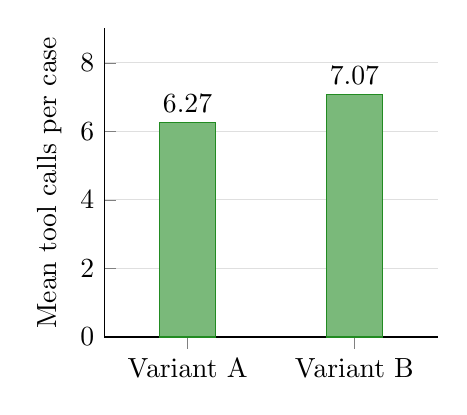
\begin{tikzpicture}
\begin{axis}[ybar,bar width=20pt,width=0.48\linewidth,height=5.5cm,
  ymin=0,ymax=9,ylabel={Mean tool calls per case},
  symbolic x coords={Variant A,Variant B},xtick=data,
  nodes near coords,nodes near coords align={vertical},
  every node near coord/.append style={/pgf/number format/fixed,/pgf/number format/precision=2},
  enlarge x limits=0.5,axis lines*=left,ymajorgrids,grid style={gray!25}]
\addplot[fill=ForestGreen!60,draw=ForestGreen] coordinates {(Variant A,6.27) (Variant B,7.07)};
\end{axis}
\end{tikzpicture}
\caption{Verdict accuracy (left) and mean tool calls per case (right) for the two variants}
\label{fig:ab}
\end{figure}

The accuracy of both variants was identical in all three repetitions, because the system is
deterministic; the variation between repetitions is confined to latency. Per-repetition mean latencies
were 11.3, 14.4 and 15.4\,ms for variant~A and 20.7, 13.8 and 15.8\,ms for variant~B. The first
repetition of variant~B includes one case of 391.5\,ms caused by start-up work, which raises that
repetition's mean; the difference in mean latency between the variants is therefore of the same order
as the variation between repetitions.

All nine cases on which the variants differ are cases in which the first iteration could not resolve
the product: in variant~A they end as \emph{Insufficient evidence}, six of which should have been
\emph{Supported} and three \emph{Conflicting}. Variant~B re-plans on exactly these nine cases and on no
others; each re-planned case executes ten nodes and eleven tool calls instead of six nodes and five to
seven tool calls.

\section{Discussion and Decision}

The hypothesis was supported on all three counts. The re-planning loop increased verdict accuracy by
20 percentage points, from 80.0\% to 100.0\%, and macro-F1 from 0.80 to 1.00. It introduced no false
\emph{Supported} verdicts, because the second iteration only resolves names that match a registered
alias and still requires every check to pass. Its cost was 0.8 additional tool calls per case on
average and an increase in mean latency of about 3\,ms, far below the one-second bound and comparable
to the run-to-run variation.

The experiment also shows where the benefit comes from. Variant~A is not unsafe: it never endorses a
false claim and it abstains on all unclear cases. Its weakness is that it abstains too often, sending
24 cases to human review instead of the 15 that genuinely require it. The loop therefore reduces the
workload of human reviewers by nine cases out of 45 (20\%) without lowering safety. In a deployment
where reviewers are the scarce resource, this is the most important effect.

Two cautions apply. First, the result was obtained on a test set in which six of 45 cases deliberately
use aliases; the size of the benefit depends on how often real labels use non-registered names. Second,
Chapter~7 showed that names outside the alias list are not resolved even with re-planning, so the loop
helps only as far as the alias table and matching rules allow. \textbf{Decision:} variant~B, with a
maximum of three planning iterations, was adopted as the default configuration, because it improves
accuracy and reduces reviewer workload at negligible cost and with no loss of safety.
